\textbf{Problem 3 Project}\\
facebook data set - project not finished (not enough time left)\\
\textsl{This projects tries to answer several questions like it is mentioned in the suggestions.}\\
	\textsl{a) Do all given ego-networks merge together in one larger network?}\\
	\textsl{b) Are the base-nodes (or ego-nodes) for the ego-networks the most important in the merged network? Are there more important nodes?}\\

\textbf{Solution}:\\
The data set represents 10 users with their friends on the facebook network\cite{facebook_data}. The data is stored in several files. The connections between one node and its friends is stored in the nodeId.edges files. The data in these files contains the edges (or friendships) between the nodeId's sub-nodes (or friends). By doing that, the network is split into several "ego-networks". By merging the 10 .edge files and adding the connections between ego-nodes and their friends, we receive the whole network for this project.\\

The question a) states, that all sub-graphs are connected. This can be assumed due to the small introduction, but shall be proven visually in this matter. The graph can be seen in figure \ref{fig:facebook_network_global}. Without any further explanation we see that there are no nodes which are not connected within the network.\\

\begin{figure}[h]
	\centering
	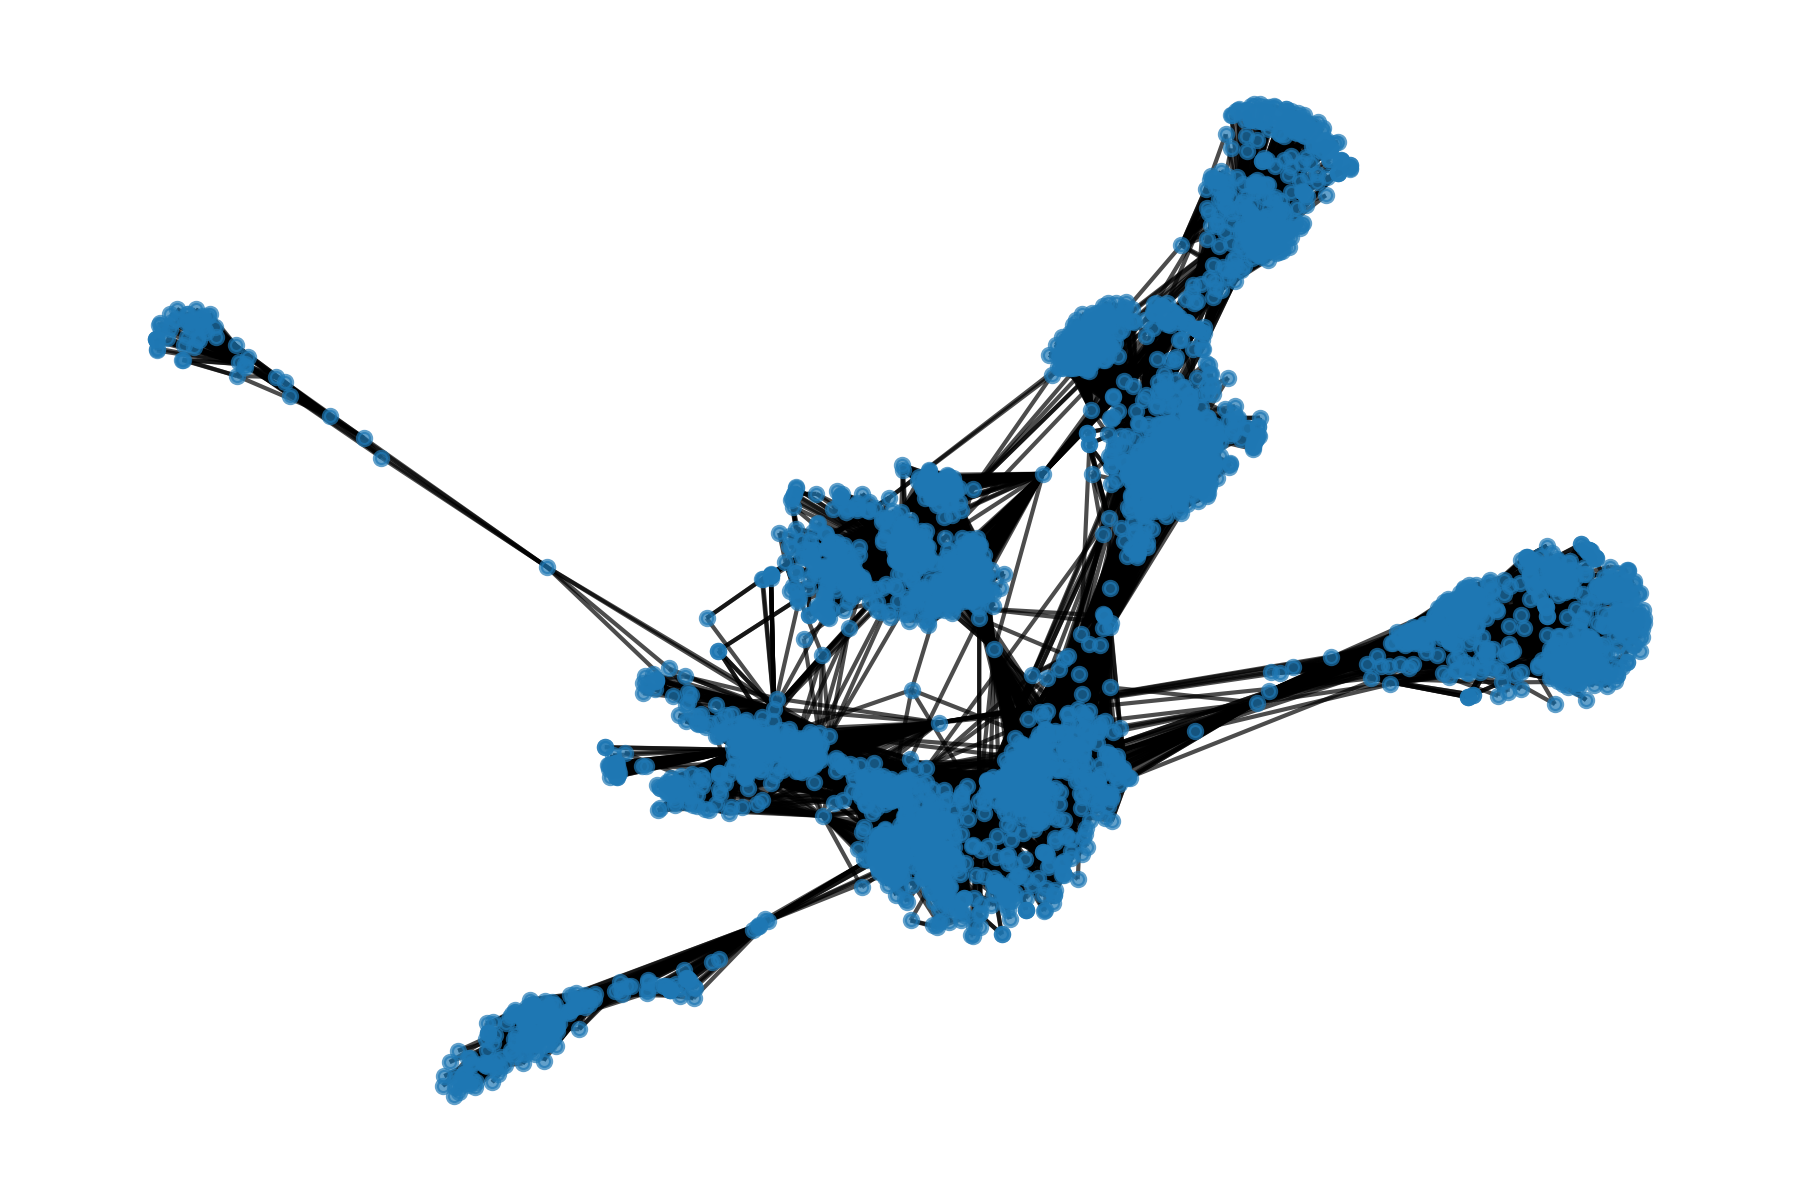
\includegraphics[width=0.7\linewidth]{problem_03/facebook_network_global}
	\caption{Connected nodes (10 representative nodes with their ego-networks)}
	\label{fig:facebook_network_global}
\end{figure}

To answer question b) we need to define on which criterion the importance of a node is defined. We have several possibilities for this definition. To answer the question I will list the ego-nodes, ordered by importance according to the ego-network node count or the degree of the ego-node\footnote{Due to the undirected network, the in-degree is equivalent to the out-degree.}. Next, I will compare this list with the degree of all nodes, the eigenvector and the betweenness centrality of the 10 nodes of highest centrality.\\

As the table \ref{tab:importance_nodes} shows, the ego-nodes are not necessarily the most important nodes according to the before mentioned centrality measures. The degree is a poor criterion to judge whether other nodes are more important than ego-nodes. Nodes in larger ego-networks generally reach higher degrees, irrelevant if the node is an ego-node or a plain sub-node within the ego-network due their numerous connections. 

\begin{table}[h]
	\centering
	\begin{tabular}{|c|c|}
		\hline 
		Degree (ego-nodes) 	& Degree (all nodes)\\ 
		$[$edge count$]$ 	& $[$edge count$]$\\ 
		\hline 
		no.107 (1034) 		& no.107 (1034)\\ 
		\hline 
		no.1684 (786) 		& no.1684 (786)\\ 
		\hline 
		no.1912 (747)		& no.1912 (747)\\ 
		\hline 
		no.3437 (534) 		& no.3437 (534)\\ 
		\hline 
		no.0 (333)    		& no.0 (333)\\ 
		\hline 
		no.348 (226)  		& no.2443 (294)\\ 
		\hline 
		no.686 (168)  		& no.2347 (291)\\ 
		\hline 
		no.414 (150)  		& no.1888 (254)\\ 
		\hline 
		no.698 (63)			& no.1800 (245)\\ 
		\hline 
		no.3980 (52)		& no.1663 (235)\\ 
		\hline 
	\end{tabular} 
	\caption{Comparison of different nodes according to importance (left to right: degree of ego-nodes and all nodes, (missing: eigenvector centrality, betweenness centrality))}
	\label{tab:importance_nodes}
\end{table}